% !TEX root = ./Basilisk-planetEphemeris-20190422.tex


\begin{figure}[h]
	\centerline{
		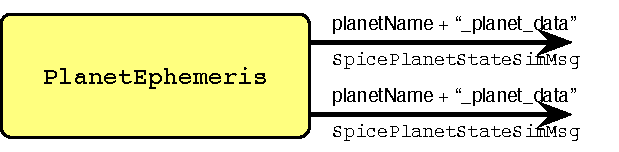
\includegraphics{Figures/moduleImg}
	}
	\caption{Illustration of the module input and output messages.}
	\label{fig:moduleImg}
\end{figure}


\section{Model Description}
The purpose of this module is to create planetary ephemeris messages where the planetary motion is modeled through classical orbit elements.  The module output messages are illustrated in Figure~\ref{fig:moduleImg}.  Note that there are no input messages.  The planetary translational motion, and optionally the rotational motion, are specified through the module parameters directly.  


\subsection{Specifying the required planetary translational information}
The first step is to specify the planet names that are to be modeled.  This is done by creating a C++ vector of strings and setting them using the module {\tt setPlanetNames()} method.  The length of this vector determines how many output messages are created in the vector {\tt planetOutMsgs}.  The planet name string provided is used to fill the output message {\tt PlanetName} variable.

Next the translational planetary motion is specified through a C++ vector of classical orbit element structures called {\tt planetElements}.  The true anomaly provided is assumes to be the anomaly angle at epoch.  This is the same time as the zero'th simulation time step. 






\subsection{Specifying the optional planetary orientational information}
The planet orientation information is optional.  However, if it is specified for one planet it must be specified for all planets.  The planet polar rotation axis $\hat{\bm e}$, i.e. the 3rd axis of the planet fixed frame, is specified through the right ascension angle RAN and declination angle DEC using
\begin{equation}
	\leftexp{N}{\hat{\bm e}} = \leftexp{N}{\begin{bmatrix}
		\cos(\text{RAN}) \cos(\text{DEC}) \\
		\sin(\text{RAN}) \cos(\text{DEC}) \\
		\sin(\text{DEC})
	\end{bmatrix}}
\end{equation}

The initial angular rotation about this axis is given by the local sidereal time (LST) angle $\gamma_{0}$ at the epoch time.  The LST at the current time is determined using the planet's polar rotation rate $\omega_{P/N}$:
\begin{equation}
	\gamma(t) = \gamma_{0} + \omega_{P/N} (t - t_{\text{epoch}})
\end{equation}
From these states the planet's DCM $[PN]$ and DCM rate $[\dot{PN}]$ are evaluated.

If the planet orientation information is computed, then the output message {\tt computeOrient} is set to +1.  If not, then {\tt computeOrient} is 0.  If the orientation is not specified, then the planet DCM is set to the identity matrix with $[PN] = [I_{3\times 3}]$.  The DCM rate is set to zero.  If any orientation states are not specified, then the module will output this default zero orientation attitude.  